%!TEX root = P231_notes.tex

\section{Linear Algebra Review}

As physicists, linear algebra is part of our \acro{DNA}, from the vector calculus in our first electrodynamics course to quantum mechanics. So why should we patronize ourselves with yet another review of linear algebra?
%
We want to understand Green’s functions the inverse of a matrix. The `matrix' in question is the differential operator $\mathcal O$ in \eqref{eq:greens:function:equation}.
%
This is important:
\begin{align}
	\text{differential operator}
	&=
	\infty\text{-dimensional matrix} \ .
\end{align}
If differential operators are matrices, what vector space do these matrices act on? These matrices act on a space of functions, which turns out to be a vector space:
\begin{align}
  \text{function space} &= \infty\text{-dimensional vector space} \ .
\end{align}
Don't be intimidated by terminology like \emph{function space}; this is just an abstract place where functions live. Just recall back to your intuition from \acronum{3D} Euclidean vector space, $\mathbb{R}^3$: any 3-vector $\vec{v}$ lives in the vector space $\mathbb{R}^3$. If we transform $\vec{v}$ by a linear transformation ${A}$, you get a new vector  $\vec{w} = {A}\vec{v} \in \mathbb{R}^3$ that is also in the vector space.

%
Weird things can happen when we extend our intuition from finite things to infinite things\footnote{For example, the Hilbert Hotel puzzle.}, but for this course we'll try to draw as much intuition as we can from finite dimensional linear algebra to apply it to infinite dimensional function spaces.

\subsection{The basics}

A \textbf{linear transformation} $A$ acts on a vector $\vec{v}$ as $A\vec{v}$. 
This transformation satisfies
\begin{align}
  A(\alpha \vec{v}+ \beta \vec{w}) = \alpha A\vec{v} + \beta A\vec{w} \ .
\end{align}
Here $\alpha$ and $\beta$ are numbers.
%
This is conventionally matrix multiplication. The result is also a vector. One way that we like to think about vectors is as columns of elements:
\begin{align}
  \begin{pmatrix}
    v^{1} \\ v^{2} \\ \vdots \\ v^{N}
  \end{pmatrix} \ ,
  \label{eq:vector:def:as:column}
\end{align}
where $N$ is the \textbf{dimension} of the vector space. Our notation is that $v^i$ refers to the $i^\text{th}$ component of $\vec{v}$. Sometimes---as physicists---we refer to $v^i$ as the vector itself, which is a slight abuse of notation that occasionally causes confusion.

In this course we always assume a nice orthonormal basis. In this case, $(\vec{v} + \vec{w})^i = v^i + w^i$.
\begin{exercise}
Convince yourself that adding vectors becomes more complicated in polar coordinates. Namely, $(\vec{v} + \vec{w})^i \neq v^i + w^i$.
\end{exercise}

Because the linear transformation of a vector is another vector, we know that the sequential application of linear transformations is itself a linear transformation. This is a bombastic way of saying that you can multiply matrices to produce a matrix.  Here’s how it works in two dimensions. A transformation that takes vectors into vectors takes the following form:
\begin{align}
  A &= 
  \begin{pmatrix}
   A^{1}_{\phantom{1}1} & A^{1}_{\phantom{1}2}
   \\
   A^{2}_{\phantom{1}1} & A^{2}_{\phantom{1}2}
  \end{pmatrix} \ .
\end{align}
We have introduced upper and lower indices; for now treat this as a definition. This sometimes causes confusion. So here are some guidelines:
\begin{itemize}
	\item Treat the upper and lower indices as a definition. The components of the linear transformation $A$ are \emph{defined} by $A^i_{\phantom{i}j}$ where $i$ is the row number and $j$ is the column number. 
	\item We have not yet explained the significance of the heights, but for now we mandate that the first index is always upper and the lower index is always lower. The following objects do not (yet) make sense: $A^{1}_{\phantom{1}2}$ and \emph{not} $A_{12}$, $A^{12}$, or $A_{1}^{\phantom{1}2}$.
	\item We will soon define \emph{additional machinery} to raise and lower indices shortly. This is takes us from a vector space to a metric space.
	\item The heights of the indices are a convenient shorthand notation that we will elucidate shortly; it is related to the choice of upper indices in \eqref{eq:vector:def:as:column}.
	\item All of this may be familiar from special relativity. Extra credit if you realize that this should also be familiar from quantum mechanics.
\end{itemize}
If you’re squeamish about the indices, don’t worry: the elements of $A$ have two indices, the first one is written a little higher than the second one. This notation is neither mathematics nor physics, it’s a convention that we use for future convenience.

The action of a linear transformation $A$ on a vector $\vec{v}$ is:
\begin{align}
  A\vec{v}
  =
  \begin{pmatrix}
    A^{1}_{\phantom{1}1} & A^{1}_{\phantom{1}2}
   \\
   A^{2}_{\phantom{2}1} & A^{2}_{\phantom{2}2}   
  \end{pmatrix} 
  \begin{pmatrix}
    v^1\\
    v^2
  \end{pmatrix}
  =
  \begin{pmatrix}
    A^1_{\phantom{1}1} v^1 + A^1_{\phantom{1}2}v^2\\
    A^2_{\phantom{2}1} v^2 + A^2_{\phantom{2}2}v^2
  \end{pmatrix} \ .
\end{align}
Look at this carefully. The components of the new vector $(A \vec{v})^i$ are sums. In each term, the second/lower index of an $A$ element multiplies the component of $\vec{v}$ with the same index. The first/upper index of $A$ tells you whether that term should is in $(A \vec{v})^1$ or $(A \vec{v})^2$. 

A generic component of $(A\vec{v})$ is
\begin{align}
  (A\vec{v})^i = \sum_j A^i_{\phantom{i}j} v^j
  = A^i_{\phantom{i}j} v^j \quad \text{(Einstein convention)}
   \ .
\end{align}
On the right-hand side we use Einstein notation: \emph{we implicitly sum over repeated upper/lower indices}. We will use this notation from now on.
%
If you are at all in doubt about this, please work out the $2\times 2$ case carefully and compare to the succinct notation above. 

\begin{exercise}
Consider three-dimensional Euclidean space, $\mathbb{R}^3$. A linear transformation $A$ on this space is a $3\times 3$ matrix with elements of the form $A^i_{\phantom{i}j}$. Explicitly write out the second component of the vector $A\vec{v}$. This is a sum of three terms.
\end{exercise}

If $A$ and $B$ are linear transformations, then $A+B$ is a linear transformation. The components of $A+B$ are simply the piecewise sum of the corresponding components of $A$ and $B$:
\begin{align}
  (A+B)^i_{\phantom i j} = A^i_{\phantom i j} + B ^i_{\phantom i j} \ .
\end{align}


\subsection{Linear Transformations and Vector Spaces}

Let’s be a little more pedantic. We need to move past the idea that a vector $\vec{v}$ is some \emph{column of numbers}. A vector space is abstract and we need to to start thinking of vector spaces more generally. The layer of abstraction is encoded in the basis vectors, which we write as $\vec{e}_{(i)}$. For a space of dimension $N$, there are $N$ such vectors indexed by the subscript. Let us more formally write the vector $\vec{v}$ as
\begin{align}
  \vec{v} = 
  v^1 \vec{e}_{(1)}
  +
  v^2 \vec{e}_{(2)} + \cdots
  = v^i \vec{e}_{(i)} \ .
  \label{eq:v:v1:v2:v3}
\end{align}
These basis vectors may be unit vectors in space. In the `column of numbers' representation, they can be unit column vectors, e.g.
\begin{align}
  \vec{e}_{(1)}
  &= 
  \begin{pmatrix}
  1 \\ 0 \\ 0
  \end{pmatrix}
  &
    \vec{e}_{(2)}
  &= 
  \begin{pmatrix}
  0 \\ 1 \\ 0
  \end{pmatrix}
  &
  \cdots \ .
\end{align}
With this basis, \eqref{eq:v:v1:v2:v3} gives \eqref{eq:vector:def:as:column}
But these may be more general objects. For example, you can specify a color of light by specifying the red/green/blue content. We could have $\vec{e}_{(1)}$ be a unit amount of red light, $\vec{e}_{(2)}$ be a unit amount of green light, and $\vec{e}_{(3)}$ be a unit amount of blue light. Then a 3-vector $\vec{v}$ would correspond to light of a particular color. This color space is a vector space.




\subsection{A funny vector space: histogram space}

Here’s a funny vector space that we’re going to use as a pedagogical crutch. Imagine histogram-space. The basis vectors are:

\begin{center}
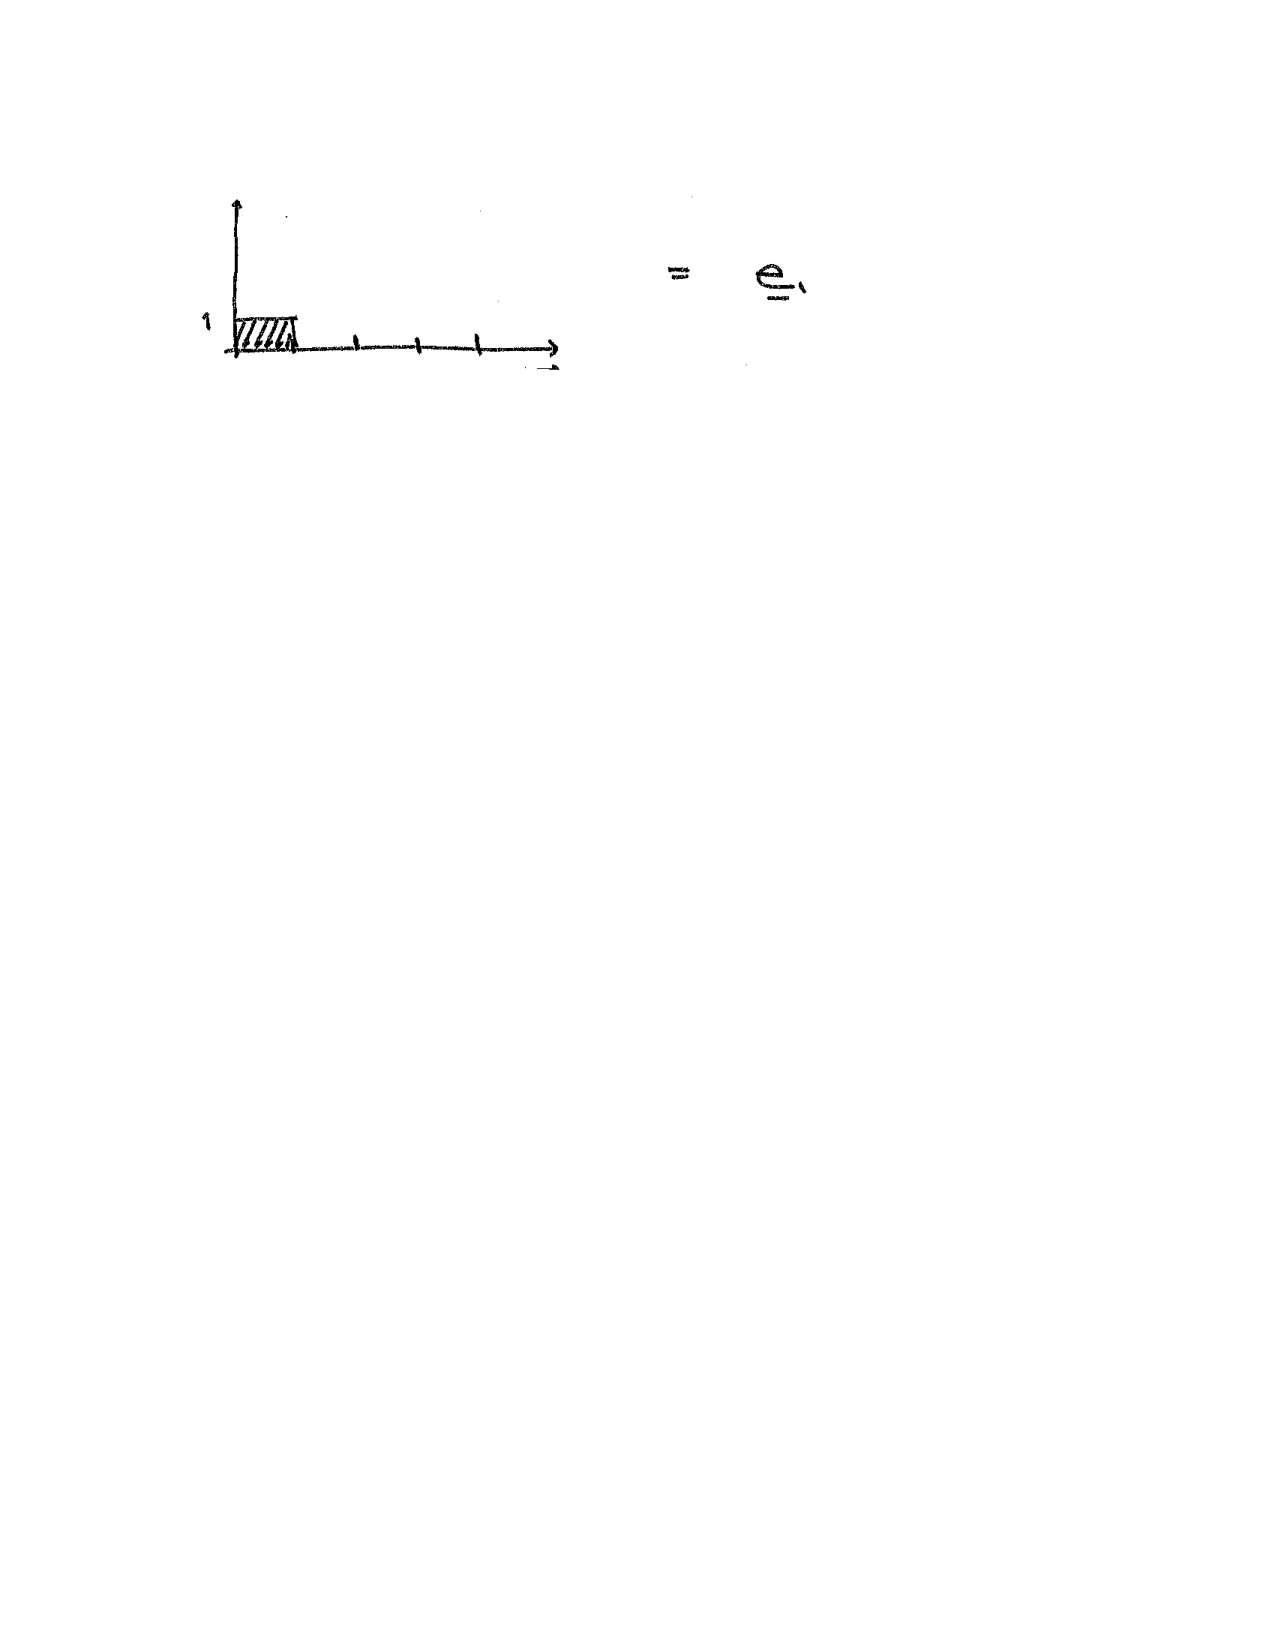
\includegraphics[width=.45\textwidth]{figures/lec02_e1.pdf}
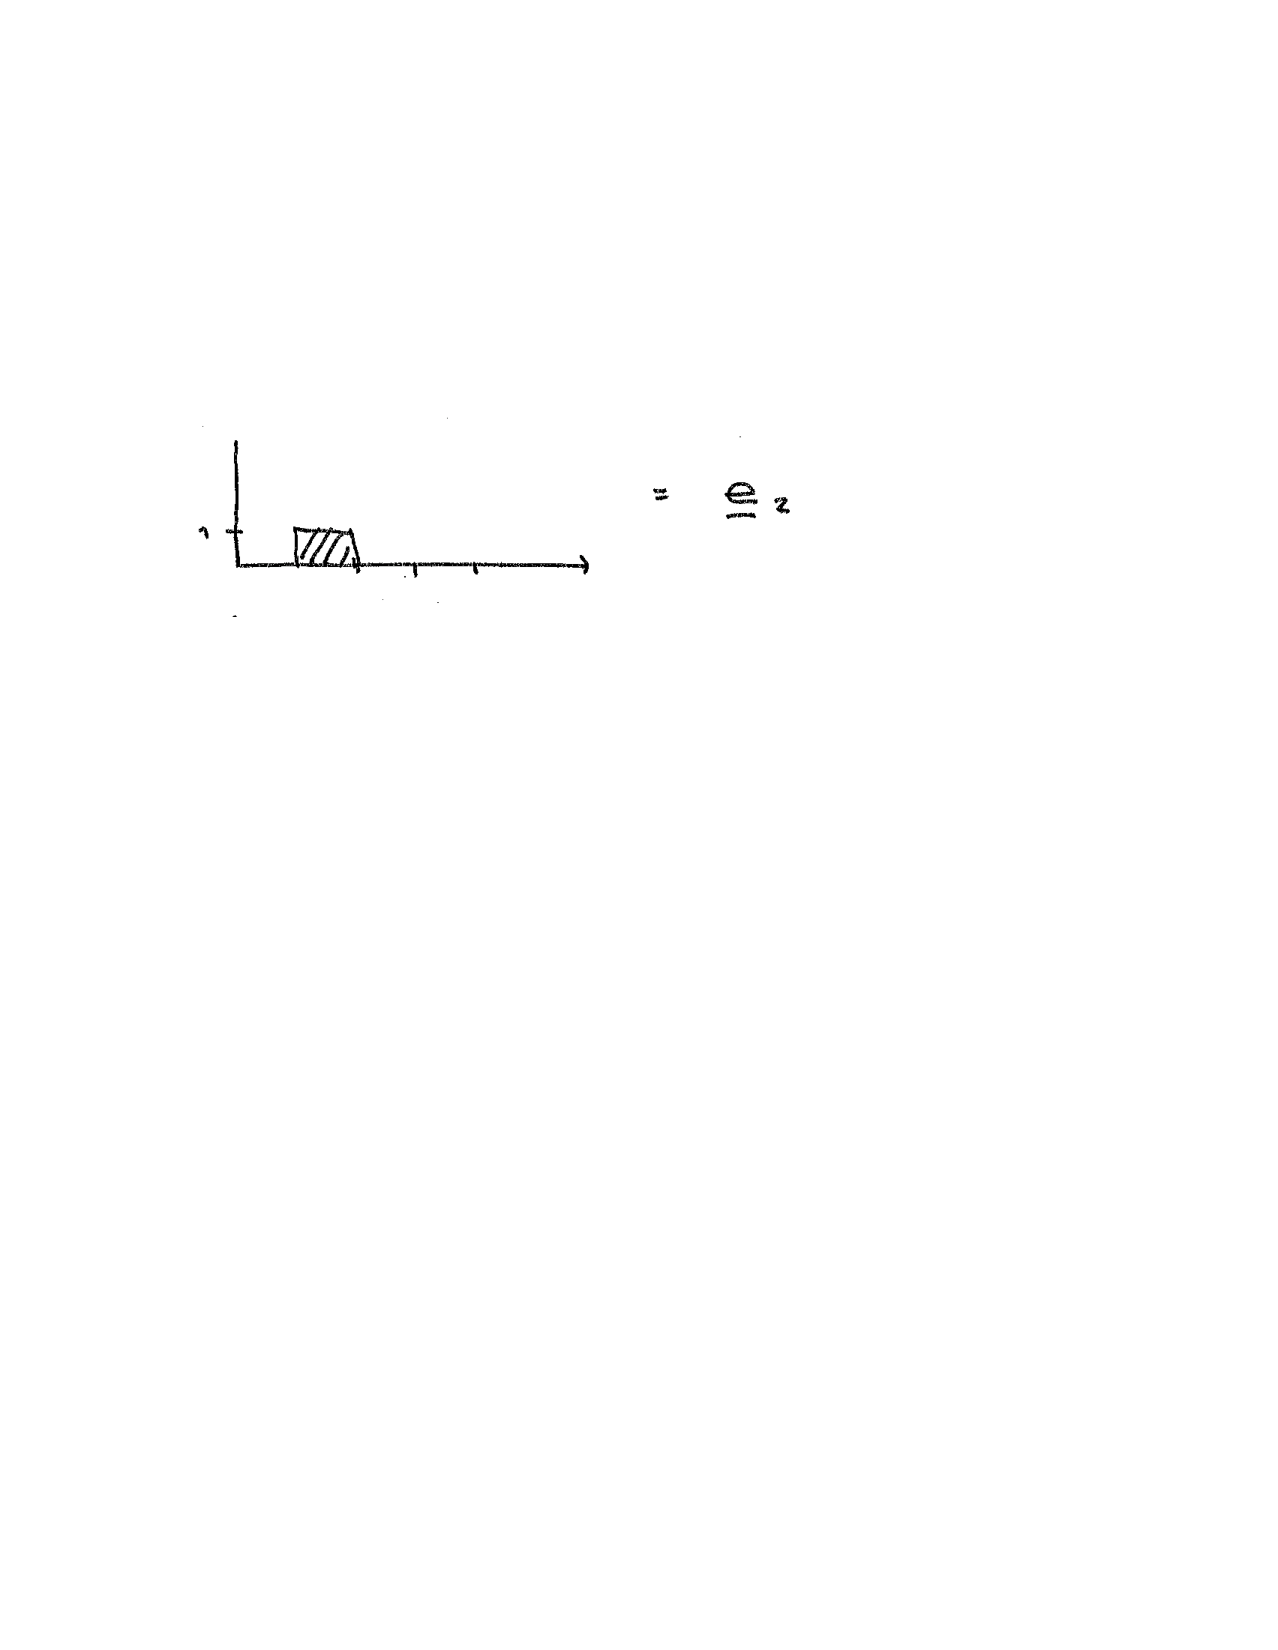
\includegraphics[width=.45\textwidth]{figures/lec02_e2.pdf}\\
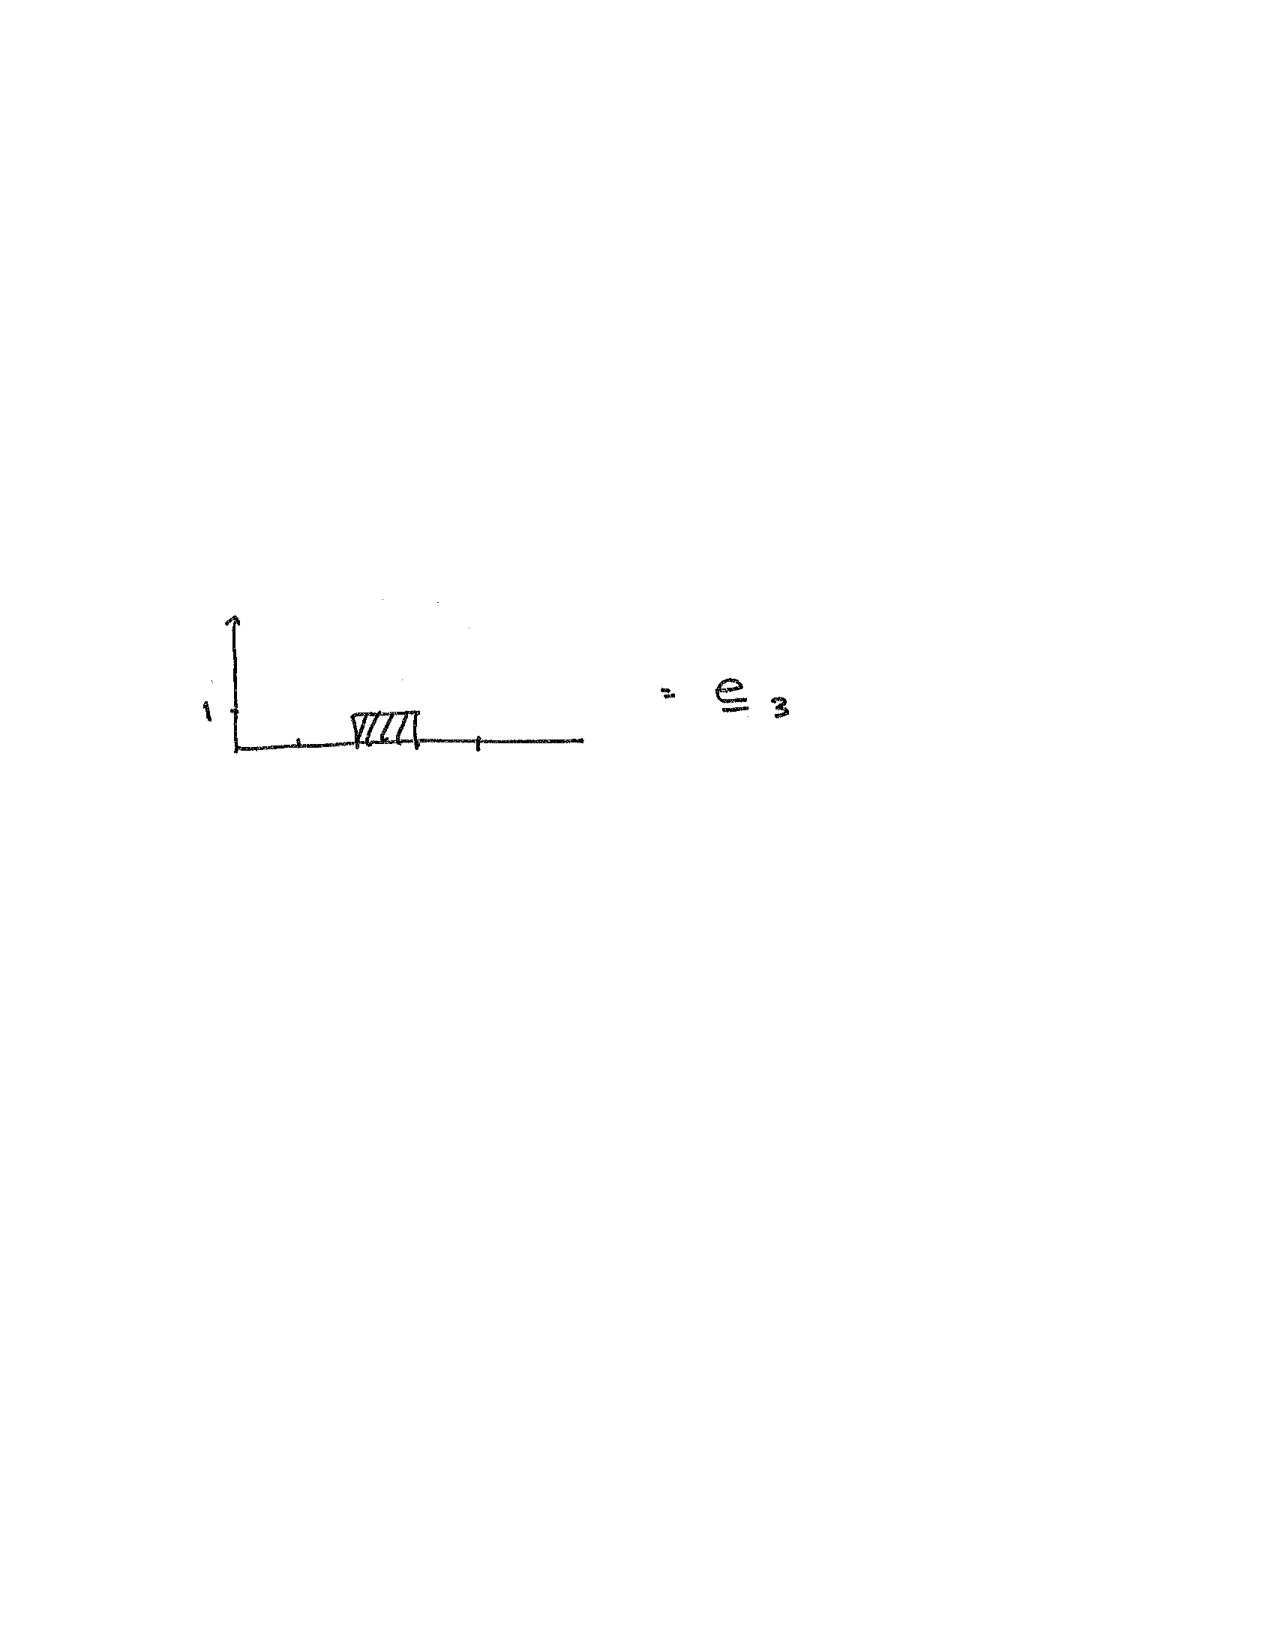
\includegraphics[width=.45\textwidth]{figures/lec02_e3.pdf}
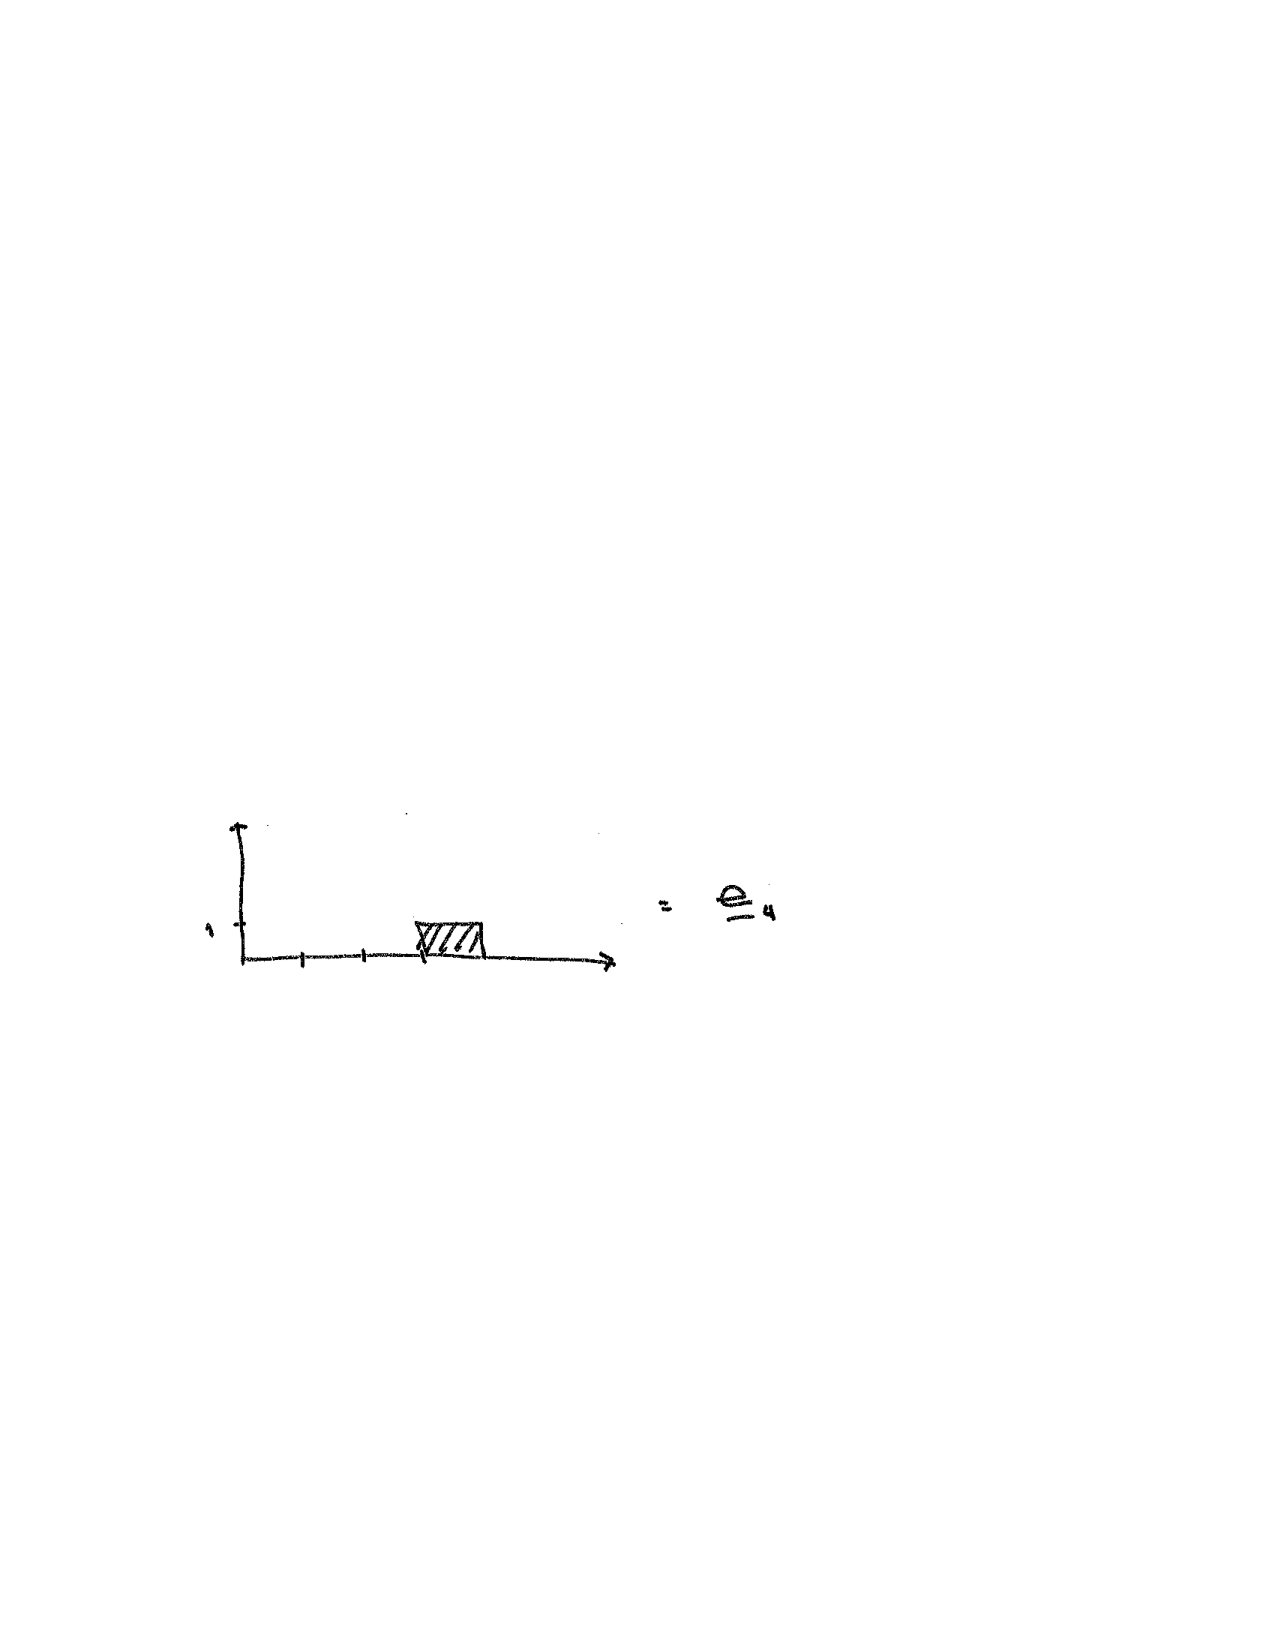
\includegraphics[width=.45\textwidth]{figures/lec02_e4.pdf}
\end{center}

\noindent This is a basis for a histogram over unit bins from $x=0$ to $x=4$. A vector in this space is, for example:

\begin{center}
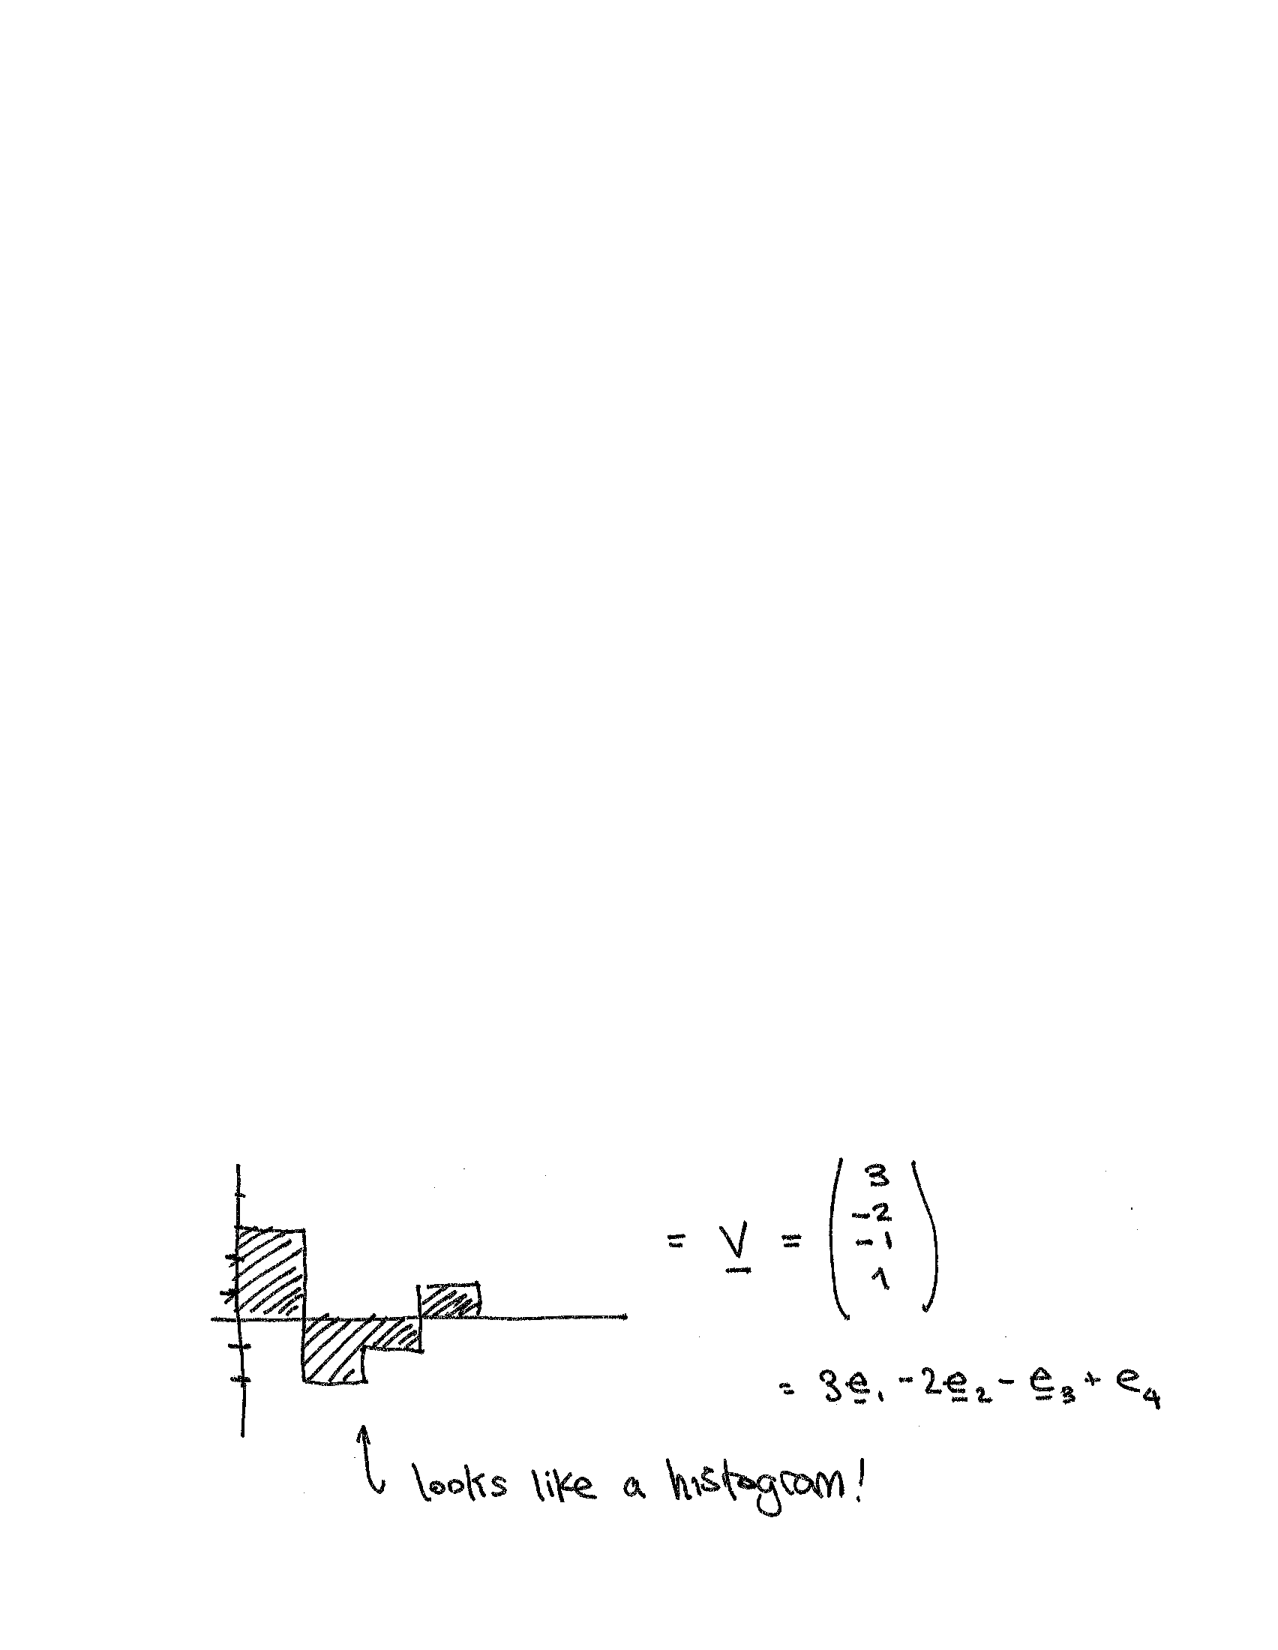
\includegraphics[width=.8\textwidth]{figures/lec02_hist.pdf}
\end{center}

\noindent We can perform a linear transformation $A$ on $\vec{v}$ which outputs another vector. Let’s say it’s this:


\begin{center}
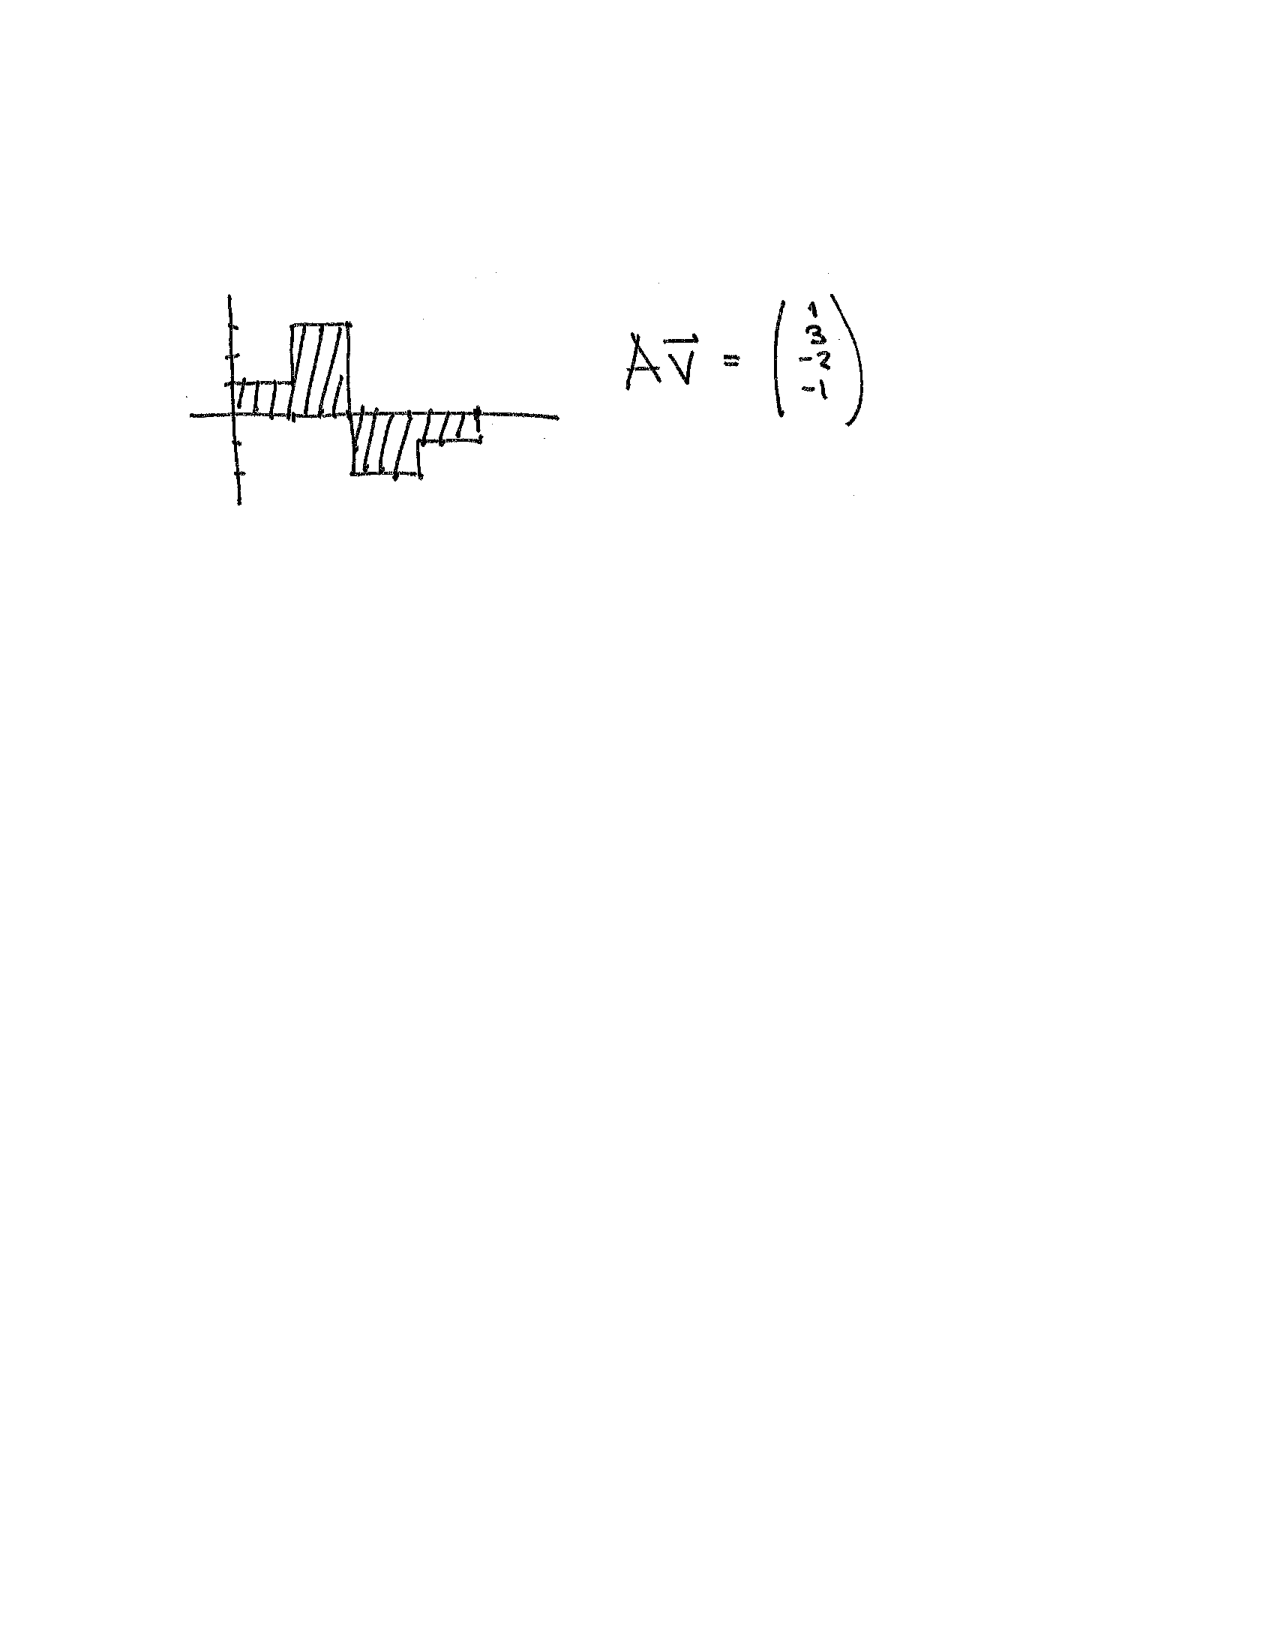
\includegraphics[width=.8\textwidth]{figures/lec02_hist2.pdf}
\end{center}

\begin{exercise}
From the image above, can you derive what $A$ is? 
\end{exercise}

\noindent The answer to the above exercise is \emph{no}. Please make sure you convince yourself why: there are many different transformations that convert to old histogram into the new histogram. If you're not convinced: the matrix $A$ is $4\times 4$ and thus has 16 entries that we need to define. The matrix equation $A\vec{v} = \vec{w}$ for known vectors $\vec{v}$ and $\vec{w}$ encodes only four equations.

The power of this admittedly strange formalism is that we can think of these histograms as approximations of continuous functions:

\begin{center}
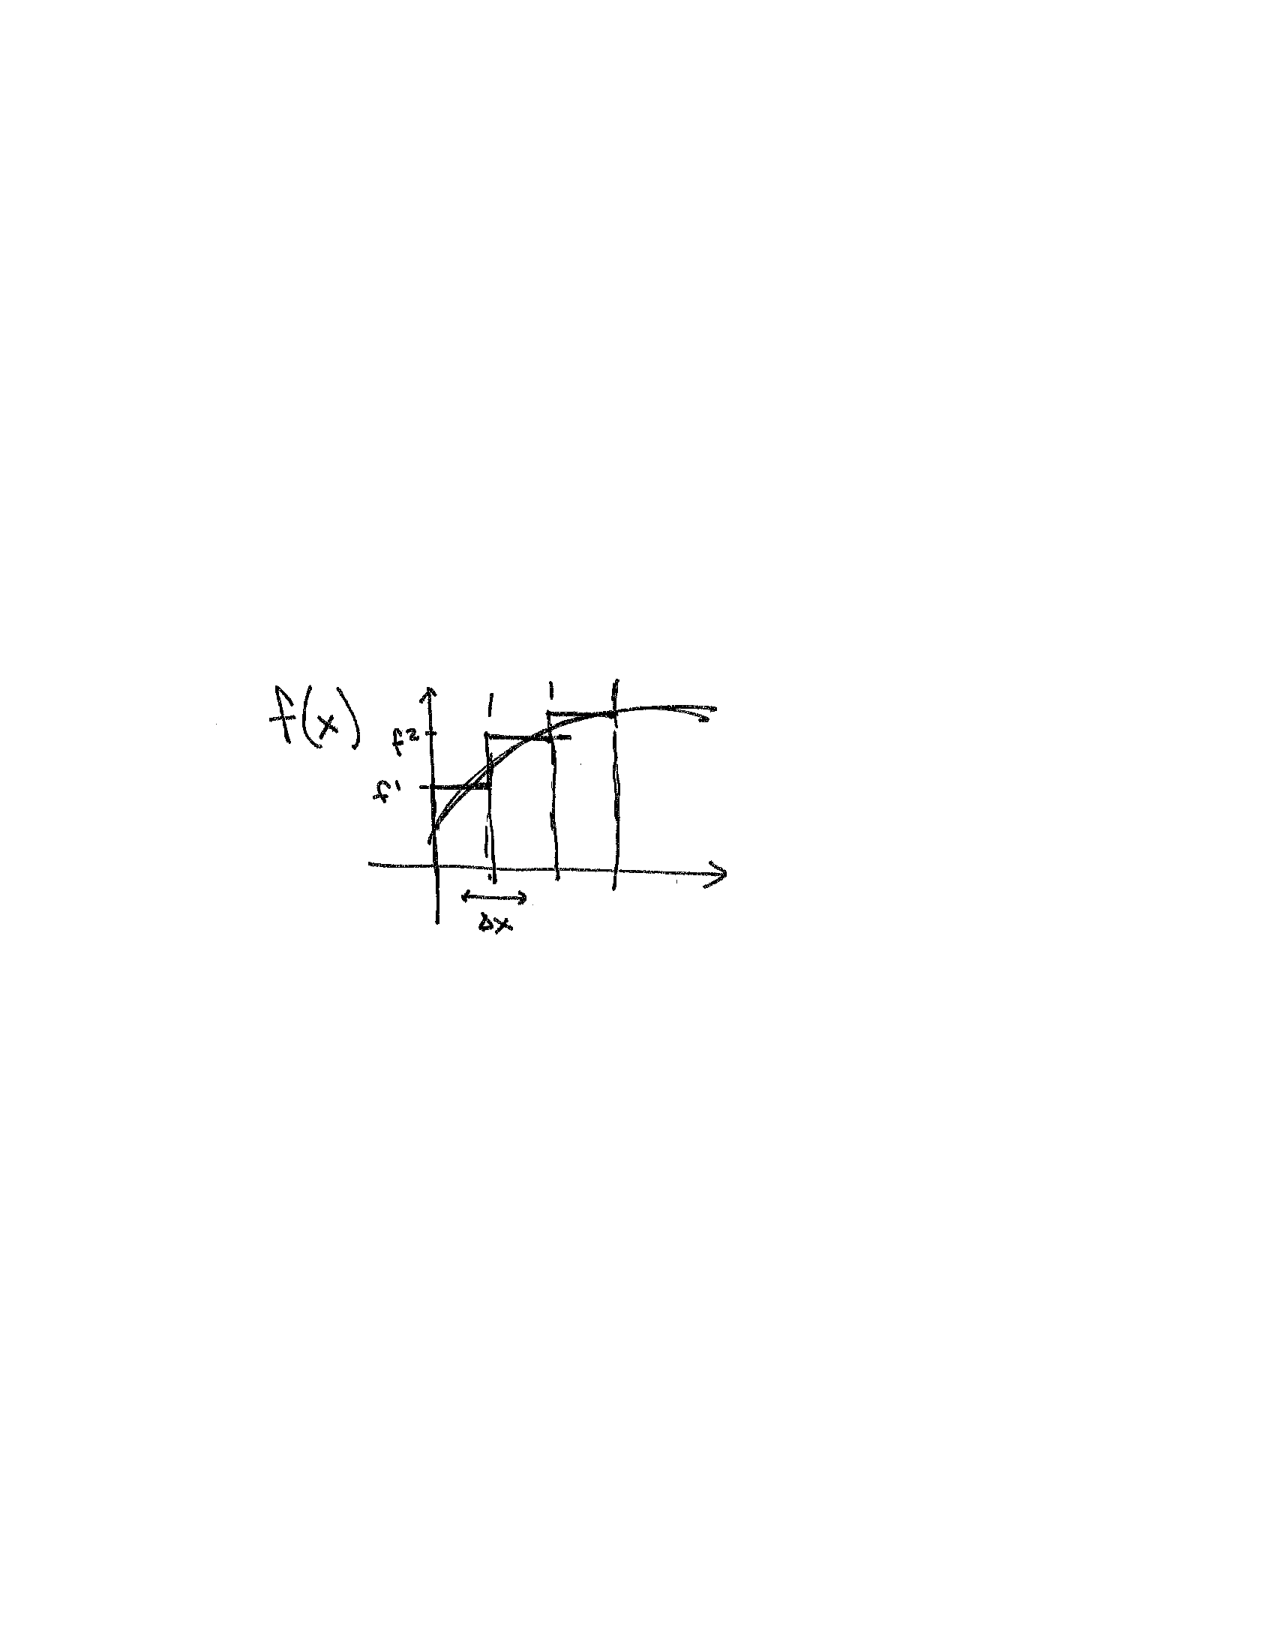
\includegraphics[width=.4\textwidth]{figures/lec02_histfun.pdf}
\end{center}

Thus a vector in this approximate (discretized) \emph{function} space is 
\begin{align}
  \vec{f} = 
  \begin{pmatrix}
    f^1 \\
    f^2 \\
    \vdots\\
    f^N
  \end{pmatrix} \ .
\end{align}

\subsection{Derivative Operators}

Our discretized function space allows us to define a [forward] derivative:
\begin{align}
  \vec{f'} =
  \frac{1}{\Delta x}
  \begin{pmatrix}
    f^2 - f^1 \\
    f^3 - f^2 \\
    \vdots
    \\
    f^{i+1}-f^i
    \\
    \vdots
  \end{pmatrix} \ .
\end{align}
This is familiar if you’ve ever had to manually program a derivative into a computer program. Note that the right-hand side looks like a linear transformation of $\vec{f}$. In other words, we expect to be able to write a matrix $D$ so that
\begin{align}
  \vec{f'} = D\vec{f} \ .
\end{align}
One problem is apparent: what happens at the `bottom’ of the vector? What is the last component of the derivative, $\vec{f'}^N$? Formally, this is
\begin{align}
  {(f')}^N = \frac{1}{\Delta x}(f^{N+1} - f^N) \,
\end{align}
but now we have no idea what $f^{N+1}$ is. That was never a component in our vector space. There is no $\vec{e}_{(N+1)}$ basis vector. 

This demonstrates and important lesson that we’ll need when we move more formally to function spaces: \emph{boundary conditions are part of the definition of the function space}. 

In the present case, let’s assume Dirichlet boundary conditions. A convenient way to impose this is to define what happens to all functions outside the domain of the function space:
\begin{align}
  f^{i > N} = f^{i < 1} = 0 \ .
\end{align}
This solves the problem of the derivative on the last component:
\begin{align}
  {(f')}^N = \frac{1}{\Delta x}(f^{N+1} - f^N) 
  = 
  \frac{- f^N}{\Delta x}  \ .
\end{align}

Alternatively, we could have also imposed periodic boundary conditions:
\begin{align}
  f^{i} &= f^{i+ kN}
  & k\in \mathbb{Z} \ .
\end{align}
This would then give
\begin{align}
  {(f')}^N = \frac{1}{\Delta x}(f^{N+1} - f^N) 
  = 
  \frac{1}{\Delta x}(f^{1} - f^N) 
  \ .
\end{align}
One could have also defined a backward derivative where $(f')^i \sim f^{i}-f^{i-1}$ \ . The second derivative may be defined symmetrically:
\begin{align}
  (f'')^i = \frac{(f^{i+1} - f^i) - (f^i - f^{i-1})}{\Delta x^2} \ .
\end{align}
You may pontificate about the reason why the first derivative does have a symmetric discretization while the second derivative does. 


\subsection{Derivatives in other function space bases}

There are other ways to write a discrete basis of functions. Here’s a natural one for functions that are up to second-order polynomials:
\begin{align}
  \vec{e}_{(0)} &= 1
  &
  \vec{e}_{(1)} &= x
  &
  \vec{e}_{(2)} &= x^2 \ .
\end{align}
Let’s sidestep questions about orthonormality for the moment. Clearly linear combinations of these basis functions can produce any quadratic function:
\begin{align}
  f(x) &= a x^2 + bx + c
  & \Rightarrow&&
  \vec{f} &=
  \begin{pmatrix}
     c \\ b \\ a
   \end{pmatrix} \ . 
\end{align}
The derivative operator has an easy representation in this space:
\begin{align}
  D = 
  \begin{pmatrix}
    0 & 1 & 0   \\
    0 & 0 & 2   \\
    0 & 0 & 0   
  \end{pmatrix} \ .
\end{align}
We can see that
\begin{align}
  D \vec{f}  &= 
  \begin{pmatrix}
     b \\
     2 a \\
     0
  \end{pmatrix} 
  &
  D^2 \vec{f}  &= 
  \begin{pmatrix}
     2a \\
     0 \\
     0
  \end{pmatrix} 
  &
  D^3 \vec{f}  &= 
  0 \ .
\end{align}
The last line is, of course, the realization that the third-derivative of a quadratic function vanishes. Feel free to attach mathy words to this like \emph{kernel}.

There are other bases that we may use for function space. A particularly nice one that we will use over and over is the Fourier basis, which we prosaically refer to as \emph{momentum space}. The basis vectors are things like sines, cosines, or oscillating exponentials. These do not vanish for any power of $D$.


\subsection{Locality}

Notice that in the histogram basis, the derivative matrix $D$ is sparse. It is zero everywhere away from the diagonal. The only non-zero elements on row $i$ are around the $i\pm 1$ column.  Higher powers of $D$ will sample further away, but the non-zero elements are always clustered near the diagonal.

This is simply a notion of locality. Remember the Taylor expansion:
\begin{align}
  f(x) = f(0) + f'(0) x + \frac{1}{2} f''(0)x^2 + \cdots \ .
\end{align}
If we think about the histogram as a discretization of a continuous function, then it is clear what the higher derivatives are doing. Given a function $f(x) = \vec{f}$, one might like to know about the function around some point $x_0$ corresponding to some index $i$. That is: $f^i = f(x_0)$. If you’d like to learn more about the function around that point, one can express the derivative at $x_0$. Thus $D\vec{f}$ says something about the slow, $D^2\vec{f}$ says something about the curvature, and so on. Because each successive power of $D$ samples terms further away from $f^i$, you can tell that these higher order terms are learning about the function further and further away from $x_0$. 

Now think about the types of differential equations that you’ve encountered in physics. They often include one or two derivatives. You hardly ever see three, four, or more derivatives. There’s a reason for this: nature appears to be local, so our mathematical models of nature have locality built in. Physics at one spacetime point should not depend on spacetime points that are far away. 

The reason for this is perhaps most elegant in special relativity. One of the key points of special relativity is that causality may be observer-dependent if two events do not occur at the same spacetime point. If we want to build causal theories of nature, then the dynamics at $x_0$ should not rely on what is happening at $x_1$, a finite distance away.\footnote{This is different from saying that information could propagate from $x_0$ to $x_1$; such propagation could come from some causal excitation of the electromagnetic field traveling every infinitesimal distance between the two positions.}


 

\subsection{Row Vectors and all that}

In high school we didn’t distinguish between row vectors and column vectors. They both seemed to convey the same information. The row vectors were just `tipped over.’ Perhaps you noticed that they follow the rules of `matrix multiplication’ act on a vector:
\begin{align}
  \begin{pmatrix}
    w_1 & w_2 & \cdots
  \end{pmatrix}
  \begin{pmatrix}
    v^1 \\
    v^2 \\
    \vdots
  \end{pmatrix}
  &= 
  w_1 v^1 + w_2 v^2 + \cdots \ .
\end{align}
In fact, this is like $\vec{w}^T$ is a function that acts linearly on $\vec{v}$: 
\begin{align}
  \vec{w}^T(\vec v) &= w_1 v^1 + w_2 v^2 + \cdots \ .
\end{align}

Indeed, let is be a bit more formal about this. This layer of formalism is uncharacteristic of our approach in this course, but this underpins so much of the mathematical structure of our physical theories that it is worth getting right from the beginning. 

Let $V$ be a vector space. It contains vectors, $\vec{v}$. Sometimes these are called contravariant vectors or kets. They have basis vectors $\vec{e}_{(i)}$. 

Now introduce a related but \emph{completely distinct} vector space called $V^*$. This is the space of \textbf{dual vectors} to $V$. A \textbf{dual vector} is what you may know as a \textbf{row vector}, a \textbf{ket}, a \textbf{covariant vector}, or a [differential] \textbf{one-form}. These are all words for the \emph{same idea}. An element of $V^*$, say $(\vec{w}^T)$ is a linear function that takes vectors and spits out numbers:
\begin{align}
  \vec{w}^T \in V^* \Rightarrow \vec{w}^T: V \to \mathbb{R} \ .
 \end{align}
Don’t think about $\vec{w}^T$ as some kind of operation on a vector $\vec{w}\in V$; at least not yet. For now the `$^T$' is just part of the name of $\vec{w}^T$. The two spaces $V$ and $V^*$ are totally different. We haven’t said anything about how to turn elements of $V$ into elements of $V^*$ or vice versa.
%
It should be clear that there is a sense of `duality’ here: the vectors $V$ are also linear functions that take a dual vector and spit out a number. 

Let us call the basis of dual vectors $\tilde{\vec{e}}^{(i)}$. This notation is cumbersome, so we’ll change to something different soon. The upper index is deliberate. The defining property of $\tilde{\vec{e}}^{(i)}$ is:
\begin{align}
  \tilde{\vec{e}}^{(i)}\left(\vec{e}_{(j)}\right) \equiv \delta^i_j \ .
\end{align}
One may check that this gives
\begin{align}
  \left(w_i\tilde{\vec{e}}^{(i)}\right)\left(v^j\vec{e}_{(j)}\right)
  = w_i v^j \delta^i_j = w_i v^i = w_1 v^1 + w_2 v^2 + \cdots \ .
\end{align}



\subsection{Orthonormal Bases}

At this point we should take a deep breath and state explicitly that we’ve been assuming an orthonormal basis. In this course we will continue to use an orthonormal basis. You may object to this and say that you used to believe in orthonormal bases until you had to write down the gradient (or worse, the Laplacian) in spherical coordinates. 

There are many things to be said about this, none of them are particularly edifying without a full discussion. With no apologies, I’ll make the following [perhaps perplexing] remarks:
\begin{enumerate}
\item There is no such thing as a `position vector.' Positions refer to some base space, whereas vectors (like differential operators) act on the tangent space at a point of that base space. 
\item A given tangent space is `nice’ and has a nice orthonormal basis. 
\item That basis may not be the same for neighboring tangent spaces (perhaps due to coordinates, perhaps due to intrinsic curvature). 
\end{enumerate}
In this course these nuances will not come up. In the rest of your life you’ll still have to deal with curvilinear coordinates. But suffice it to say that our study of function space will be nice an orthonormal. Of course, we haven’t yet given a definition of `normality.’

\subsection{Bra-Ket Notation}

There is neither any physics nor mathematics contained in a choice of notation. However, a convenient notation does simplify our lives. Let us introduce bra-ket notation. In this notation, we denote vectors by kets:
\begin{align}
  |v\rangle = v^i|i\rangle \ ,
\end{align}
where $|i\rangle = \vec{e}_{(i)}$ is the basis of vectors that span the vector space $V$. There is nothing new or different about this object,  $\vec{v} = |v \rangle$.

We denote dual vectors (row-vectors, one-forms) as bras:
\begin{align}
  \langle w | &= w_i \langle i| \ ,
\end{align}
where $\langle i | = \tilde{\vec{e}}^{(i)}$. The orthonormality of this basis is encoded in 
\begin{align}
  \langle i | j \rangle = \delta^i_j \ .
\end{align}

In bra-ket notation a linear transformation $A$ has a basis
\begin{align}
  A = A^i_{\phantom{i}j} |i\rangle \langle j| \ .
\end{align}
The notation $|i\rangle \langle j|$ is shorthand for $|i\rangle \otimes \langle j|$. If the $\otimes$ doesn’t mean anything to you, that’s fine. It doesn’t mean much to me either. Matrix multiplication proceeds as before:
\begin{align}
  A\vec{v} = A|v\rangle = 
  A^i_{\phantom{i}j} |i\rangle \langle j| v^k |k \rangle
  = 
  A^i_{\phantom{i}j}  v^k  |i\rangle \langle j|k \rangle
  = 
  A^i_{\phantom{i}j}  v^k  |i\rangle \delta^j_k
  = 
  A^i_{\phantom{i}j}  v^j  |i\rangle \ .
\end{align}
Observe that the power of the notation is clear: the object with the index $v^i$ is just a number. It commutes with everything. All of the vector-ness is carried in the basis objects: the bras, kets, and ket-bras. Those do not commute. But they have a well defined way in which kets act on bras (or vice versa).\footnote{This is where the $\oplus$ notation is handy. It keeps track of which kets/bras might hit which other bras/kets. This falls under the name of multi-linear algebra.}


\subsection{Eigenvectors are nice}

Give a sufficiently \emph{nice} linear transformation, $A$, there is a particularly convenient basis: the eigenvectors of $A$. These are kets $|\lambda\rangle$ such that
\begin{align}
  A |\lambda\rangle = \lambda |\lambda\rangle \ .
\end{align}
In other words, $A$ acts on the eigenvector by rescaling. The rescaling coefficient is the eigenvalues. For \emph{nice} transformations, there is a complete set of such vectors to span the vector space.

If you write a general vector $|v\rangle$ in terms of this eigenbasis,
\begin{align}
  |v\rangle = v^i |\lambda_{(i)} \rangle \ ,
\end{align}
Then the action of $A$ on this vector is easy:
\begin{align}
  A |v\rangle = \sum_i \lambda_{(i)} v^i |\lambda_{(i)} \rangle \ .
\end{align}
In fact, assuming that all of the eigenvalues are non-zero, even the matrix inverse is easy:
\begin{align}
  A^{-1}|v\rangle = \sum_i \lambda_{(i)}^{-1} v^i |\lambda_{(i)} \rangle \ .
\end{align}


\subsection{The Green’s Function Problem}

Going back to the big picture: recall that we want to solve differential equations of the form $\mathcal O f(x) = s(x)$. If we had a sense of the \emph{eigenfunctions} of $\mathcal O$, then we could expand $s(x)$ in a basis of those eigenfunctions and then apply $\mathcal O^{-1}$ to both sides. 

The analog is this:

\begin{center}
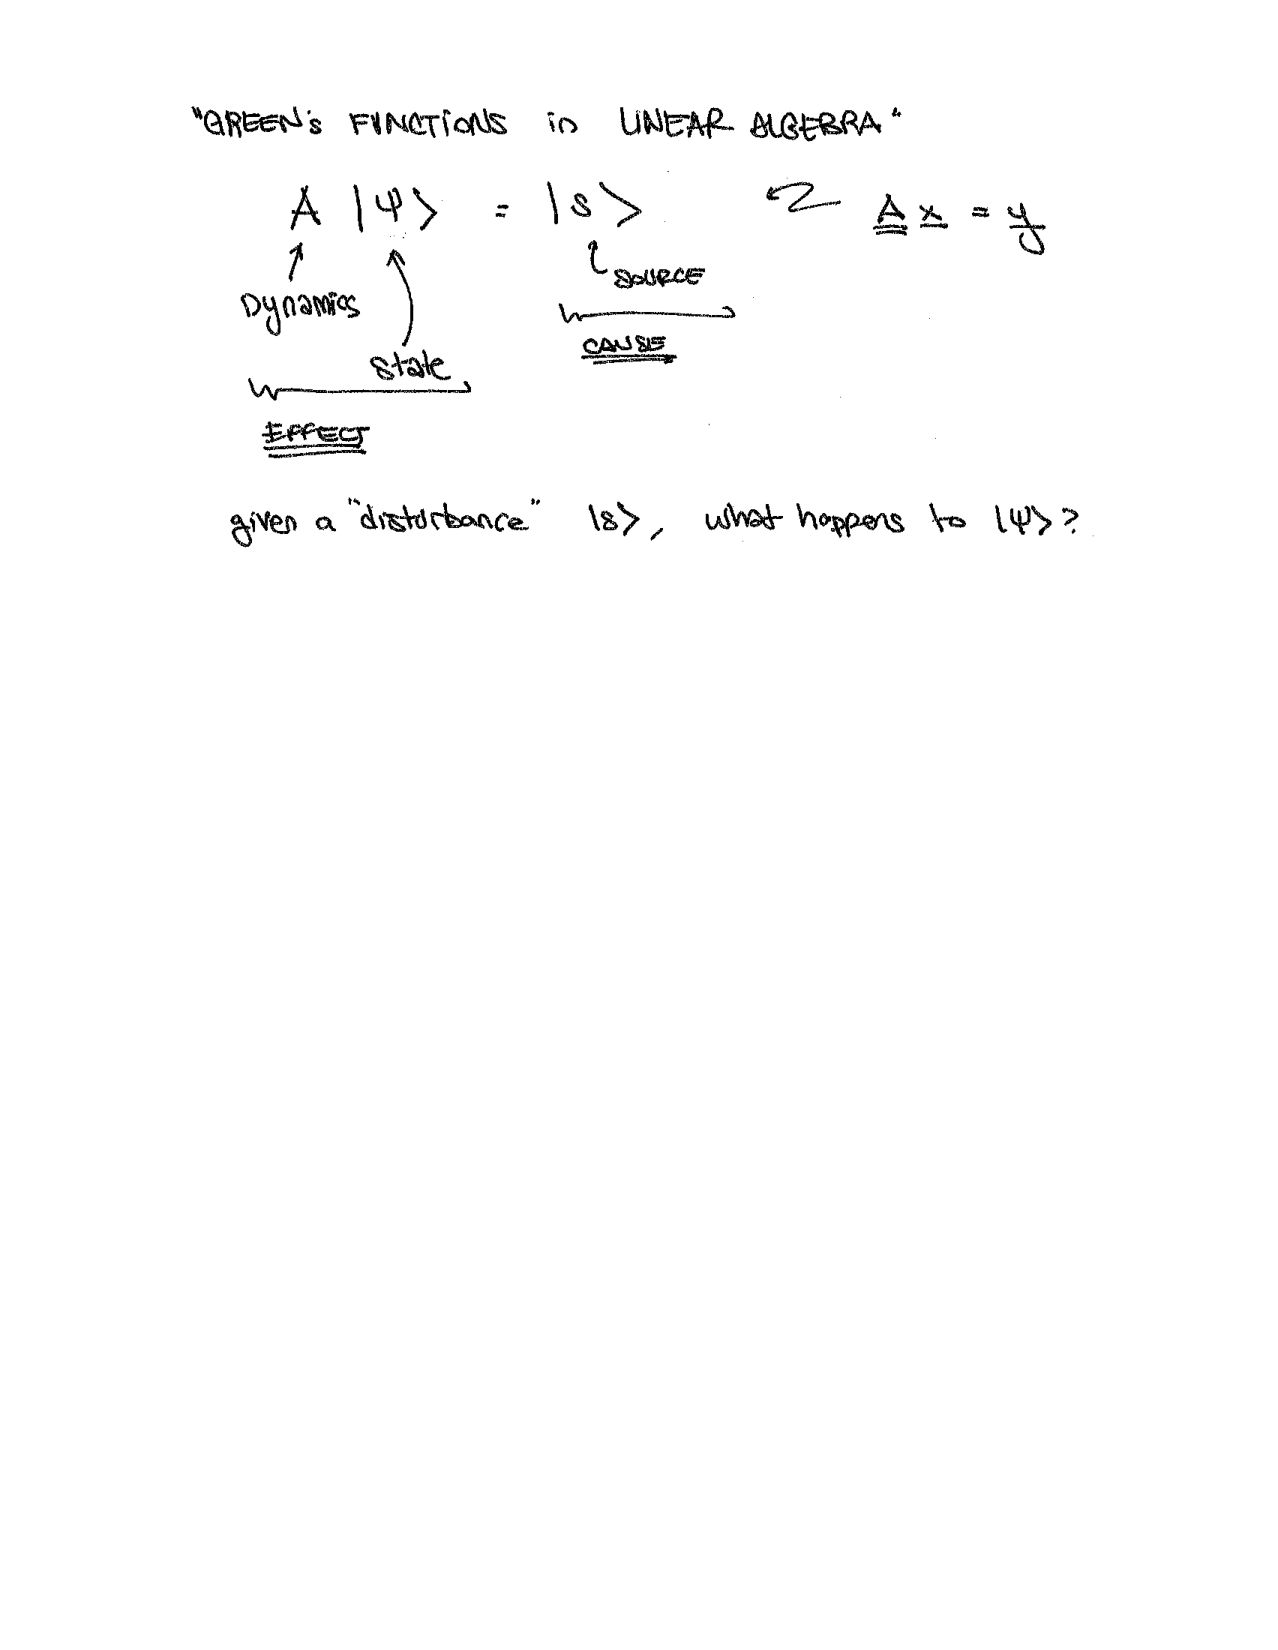
\includegraphics[width=.7\textwidth]{figures/lec02_green01.pdf}
\end{center}

 The operator $A$ encodes the \emph{physics} of the system, the underlying dynamics. This is presumably local: it is a near-diagonal matrix coming from one or two powers of derivatives.  The ket $|s\rangle$ is the source. This is the thing that \emph{causes} the dynamics. The ket $|\psi\rangle$ is some state that we would like to determine. 

\subsection{Metrics}

Thus far we have introduced vector spaces. The dual vector space is a set of linear functions that act on elements of a vector space; these are bras/row-vectors/one-forms. Let us now introduce a new piece of machinery: a \textbf{metric}. This is also known as an \textbf{inner product} or a \textbf{dot product}. A space with a metric is called a metric space. We only state this fact to emphasize that we are \emph{adding this structure by hand}. Vector spaces don‘t come with metrics---someone makes up a metric and slaps it onto the vector space.

The \textbf{metric} is a function that takes two vectors and spits out a number. It is linear in each argument. In other words, a metric $g$ is:
\begin{align}
  g:\; V\times V\to \mathbb{R} \ .
\end{align}
Occasionally one may want a metric defined such that the output is a complex number. We thus have:
\begin{align}
  g(\alpha \vec{v} + \beta\vec{w}, \delta \vec{x} + \gamma \vec{y})
  &= 
  \alpha \delta g(\vec{v},\vec{x}) + \alpha \gamma g(\vec{v},\vec{y}) + \beta\delta g(\vec{w},\vec{x}) + \beta\gamma g(\vec{w},\vec{y}) \ .
\end{align}
One more special assumption about the metric is that it is \textbf{symmetric}:
\begin{align}
  g(\vec{v},\vec{w}) = g(\vec{w}, \vec{v}) \ .
\end{align}
In indices one may write
\begin{align}
  g &= g_{ij} \langle i | \otimes \langle j |
\end{align}
so that
\begin{align}
  g(\vec{v}, \vec{w}) = g_{ij} v^{i}w^j \ .
 \end{align}
 Here we see the usefulness of the $\otimes$ notation. It tells us that the bras and kets resolve as follows:
 \begin{align}
   g_{ij}\langle i | \otimes \langle j | \left(v^k|k\rangle\right)\left(w^\ell|\ell\rangle\right) 
   = 
   g_ij v^k w^\ell 
   \langle i | k\rangle \langle j |\ell\rangle
   = 
   g_ij v^k w^\ell  \delta^i_k \delta^j_\ell 
   = 
   g_{ij} v^{i}w^j \ .
 \end{align}
 For ordinary Euclidean space in flat coordinates, the metric is simply the unit matrix: $g_{ij} = \text{diag}(1,\cdots, 1)$. In Minkowksi space there’s a relative minus sign between space and time. In curvilinear coordinates things get ugly. 
 
Here’s the neat thing about metrics. We can take a metric and pre-load it with a vector. Given a metric $g$ and a vector $\vec{v}$, we may define a function
\begin{align}
  g(\vec v,\qquad ) \ .
\end{align}
This is simply means that the function $f(\vec{w}) = g(\vec v,\vec w)$. Observe that $f(\vec{w})$ is a linear function that takes elements of $V$ and returns a number. In other words, this is a \emph{dual vector} (row-vector, one-form). Observe what having a machine like the metric has done for us: it has allowed us to convert vectors into dual vectors:
\begin{align}
  g(\vec v,\qquad )  = g_{ij} v^i \langle j| \ .
\end{align}

Similarly, one may define an inverse metric $g^{-1}$ such that $g^{-1}g = \mathbbm{1}$. In a slight abuse of notation, the inverse metric is written with two upper indices: $g^{ij}$. Note that we do not write the `$^{-1}$.' The inverse metric will \emph{raise} the index on a lower-index object, while the metric \emph{lowers} the index of an upper-index object.\footnote{Of course: what’s really happening is that the metric has a basis $\langle i|\otimes \langle j|$ while the inverse metric has a basis $|i\rangle \otimes |j\rangle$.}


\subsection{Hermitian Conjugate}

Now that we can go between column and row vectors, thanks to the metric and its inverse, it is worth thinking a bit about what we meant by the `transpose’ operator. The transpose precisely turned a column vector $\vec{v}$ into an associated column vector $\vec{v}^T$. The generalization of this idea is the Hermitian conjugate, $^\dag$. 





